\graphicspath{{chapters/02/}}
\chapter{Breakdown of classical mechanics}

\section{The fall of determinism}

  \subsection{Double slit experiment}
  The double-slit experiment is a virtual experiment, because it cannot be performed as we will describe it due to technological limitations.
  However, we can treat is as a real experiment, as it can summarize many technically feasible and performed experiments.
  The setup of this experiment consists of a gun shooting particles through a screen with two holes and a detection screen behind the first one.

  \subsubsection{Case 1 - particles are macroscopic bullets}

  \begin{figure}[h!]
    \centering
    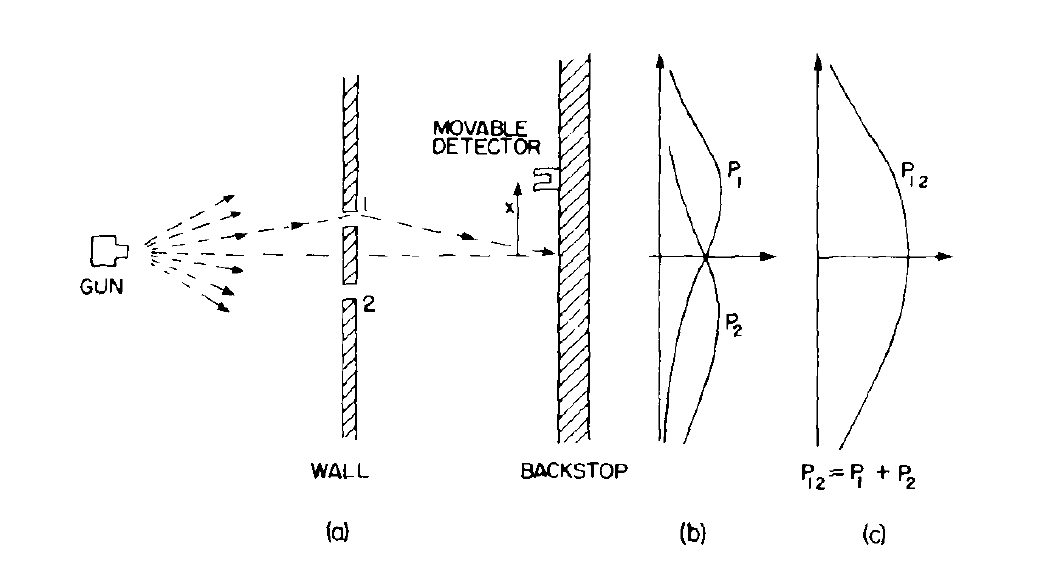
\includegraphics[clip, width=0.6\textwidth]{gun_ds.png}
    \caption{\label{fig:gun_ds} Double-slit experiment with bullets}
  \end{figure}

  In the case in which the gun shoots macroscopic bullets, we imagine the distance gun-screen to be large, implying that the bullets might arrive at different locations due to error, vibrations, wind, etc.
  Therefore, we expect bullets to arrive as a beam.

    \paragraph{Results}
    Most of the bullets will not reach the second wall, as they will remain stuck on the first one.
    However, the ones directed towards the holes will pass through.
    We expect to obtain a distribution of bullets for hole 1 and hole 2.
    If we shut down one hole 2, nothing will pass through it leading to a $p_1$ distribution.
    Conversely, if we shut down hole 1, we will observe $p_2$.
    Summarizing, we will find the following observations:

    \begin{multicols}{2}
      \begin{enumerate}
          \item bullets arrive one-by-one, we can recognize the sound of each bullet impacting the screen (if sufficient resolution is available for the recording)
          \item $P(z)$, the probability of a bullet reaching a point, can be obtained by plotting a histogram of the times a bullet has hit the point of interest. Through a statistical model we could then predict future locations.
          \item considering the experiment with one of the holes shut, a Gaussian like probability of detection $P_1$ can be seen such that $\mu$ is directly perpendicular to the hole.
          \item if both holes are open there is a \textbf{ballistic behaviour} and the resulting distribution of detection $P_{12}$ is the sum of the two deriving for each hole open by itself. As a consequence,$P_1$ and $P_2$ are disjoint events: $$P_{12} = P_1+P_2$$
      \end{enumerate}
    \end{multicols}

   \subsubsection{Case 2 - macroscopic waves in a tank}

   \begin{figure}[h!]
     \centering
     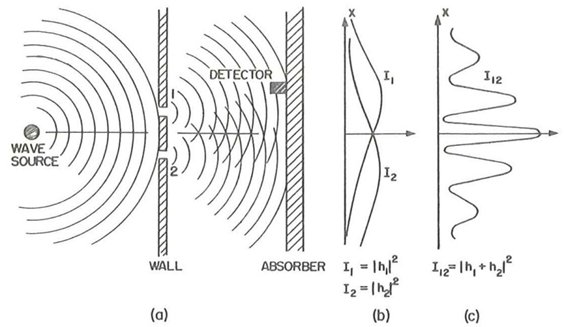
\includegraphics[clip, width=0.6\textwidth]{wave_ds.png}
     \caption{\label{fig:wave_ds} Double-slit experiment with waves}
   \end{figure}

     Suppose that rather than having a screen, we have a tank of water with a wall with two holes.
     In this case, we have an instrument producing waves e.g. something touching water.
     Since the source is very far, waves that will reach the wall will be plane waves.
     We want to measure whether the waves manage to impact the second wall.
     From each of the holes, we will observe circular waves.
     We can repeat the previous procedure of shutting each hole at a time.
     The maximum intensity (square of max amplitude) will be observed at the hole.

        \paragraph{Results}
        When the wave arrives, it reaches different locations at the same time (delocalization), very differently from bullets.
        A second difference is what we obtain when we let waves pass through both holes.
        The obtained pattern has alternating minima and maxima and it can be seen that $P_{12} \neq P_1+P_2$.
        In this case we obtain an \textbf{interference pattern}, as waves can sum and subtract in a non-trivial way (waves are complex objects).
        So, deriving from wave theory:

        $$A_1\rightarrow P_1 = |A_1|^2 = A_1^*A_1$$

        $$A_2\rightarrow P_2 = |A_2|^2 = A_2^*A_2$$

        \begin{align*}
          A_{12} = A_1+A_2\rightarrow A_{12} &= |A_1+A_2|^2=\\
                                            &=A_1^*A_1 + A_2^*A_2 + \underbrace{A_1^*A_2 + A_1A_2^*}_{\text{interference}}
        \end{align*}

        Unlike bullets, wave hit the entire screen and not at a precise time.
        This results in a wave-like behaviour with delocalization.

    \subsubsection{Case 3 - cathode as an electron gun}

    \begin{figure}[h!]
      \centering
      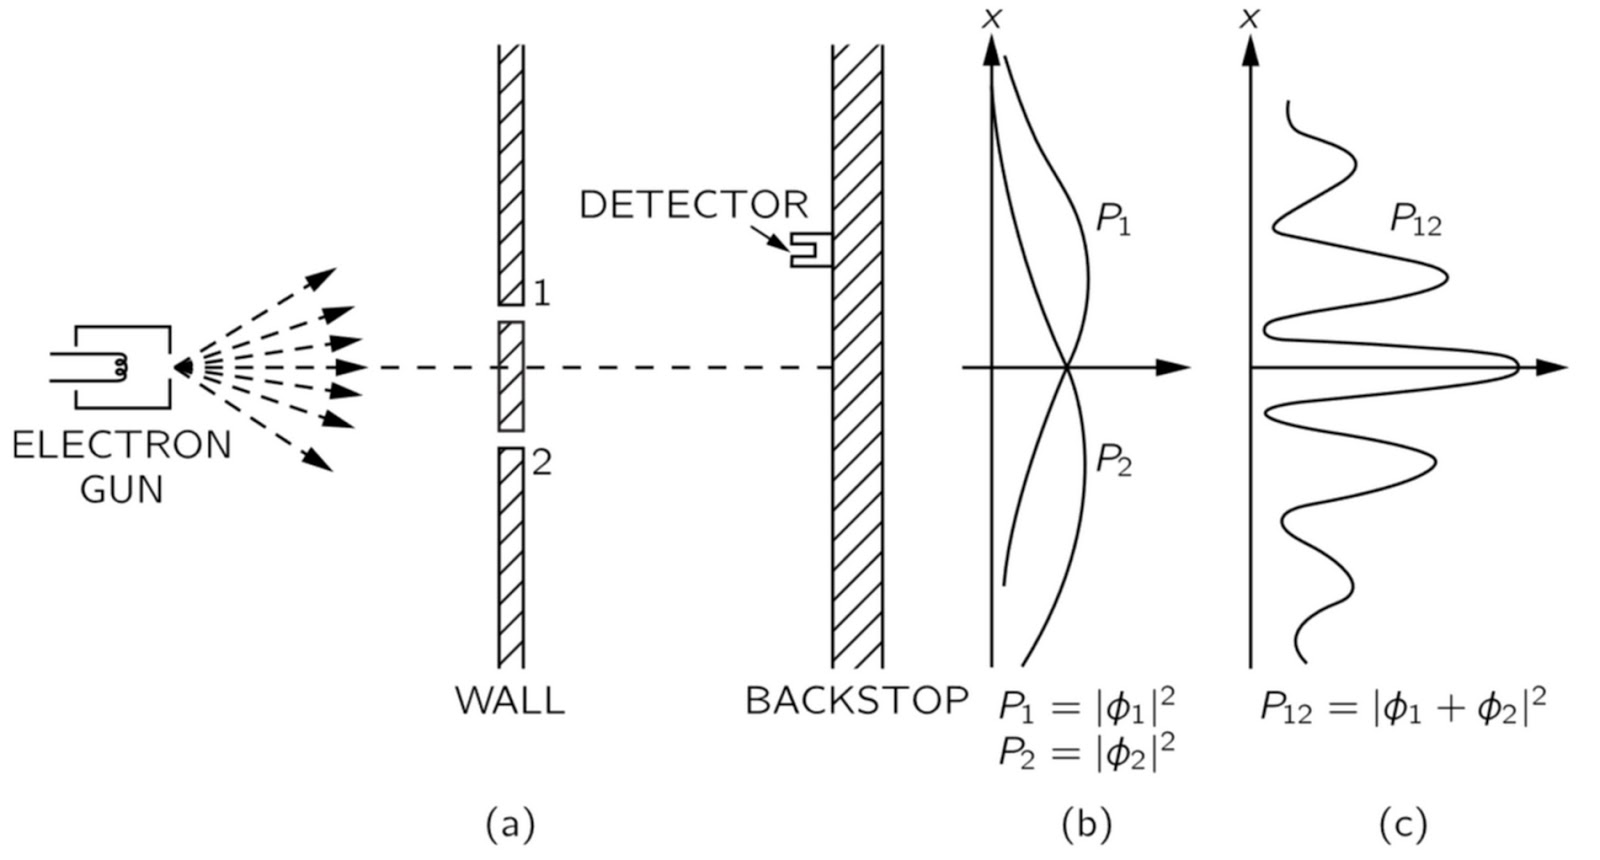
\includegraphics[clip, width=0.6\textwidth]{electron_ds.png}
      \caption{\label{fig:electron_ds} Double-slit experiment with electrons}
    \end{figure}

    Finally, let us have a cathode electron gun shooting electrons at a wall with very small holes - which need to be so small that the effect becomes evident.
    As before, we close one of the holes and the screen will record the arrival of electrons on the wall through a detector (device producing a small signal as soon as an electron arrives).
    If we place many detectors on the wall, we will retrieve when and where the electron has arrived.
    The electron signals arrive one at a time, as a "rain".
    If we open both holes, an interference pattern will be observed: $P_{tot}$ is not the sum of the single probabilities, implying that the two are not disjoint events.

      \paragraph{Results}
      Result: we observe either a \underline{particle-like behaviour} (one hole closed) or a \underline{wave-like behaviour} (both holes open).

      \paragraph{Particle detector at the holes}
      To verify whether the electron goes through both holes simultaneously, an apparatus that emits a signal if an electron travels nearby is put near the holes.
      Detection on the screen happens only if the signal is emitted.
      The two apparatuses never trigger a signal together, meaning that the electron travels through one of the holes like a particle.

      \begin{figure}[h!]
        \centering
        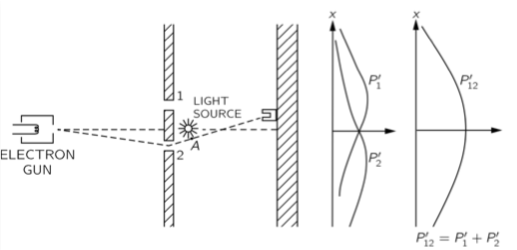
\includegraphics[clip, width=0.6\textwidth]{ele_bal_ds.png}
        \caption{\label{fig:ele_bal_ds} Double-slit experiment with electrons and apparatus emitting a signal}
      \end{figure}

      We can define $P_{A_1}$ as the probability that counts only events in which $A_1$ is triggered, and $P_{A_2}$ the results of counting only events triggering $A_2$.
      By counting all the events, it can be seen that the resulting pattern is $P_{A_1}+P_{A_2}$.
      In the case in which $P_{A_1+A_2} = P_{A_1} + P_{A_2}$, delocalization is lost and the electron assumes a \textbf{ballistic behaviour}.

      \paragraph{Summary}
      Summarizing, measurement affects the nature of the electron and can change the state of the system.
      When we try to measure where the particle goes, we observe a ballistic behaviour.
      Conversely, if we do not impose any measurement, we will obtain an interference pattern.
      The result depends on the kind of behaviour we are trying to detect.

        \subparagraph{Example}
        Suppose that we are blind. We can detect a ball by throwing something smaller at it e.g. pen cap.
        If instead we throw a pen cap towards with another pen cap, we will have a collision and both objects will end up in a different location.
        The act of measuring has changed the system!
        Throwing photons at electrons perturbs the system, as they are comparable in size.

    \subsubsection{Conclusions}
    The notion of trajectory loses significance for microscopic particles.
    This is quantified by \textbf{Heisemberg's uncertainty principle}:

    $$\underbrace{\Delta p}_{\text{Uncertainty on }p}\ \underbrace{\Delta q }_{\text{Uncertainty on }q} \ge \frac{\hbar}{2}$$

    It is impossible to simultaneously measure with arbitrary accuracy the position and the velocity of a microscopic particle.

\section{The photoelectric effect}
By considering the classical theory of the hydrogen atom and ignoring that energy loss through electromagnetic radiation would be unstable, this model can transfer any amount of energy to the electron by shining light on it.
In classical electromagnetism, the energy of radiation comes from the intensity of the electromagnetic wave.
It would be expected that, irregardless of the frequency or wave-length, the amount of electron extracted would scale with the intensity of the electromagnetic wave.

  \subsection{Experimental findings}
  Electrons are extracted only if the light has a $\nu > \nu_{\min}$ or $\lambda<\lambda_{\max}$.
  If $\nu>\nu_{\min}$, the amount of electrons scales with the intensity.
\begin{figure}[h!]
    \centering
    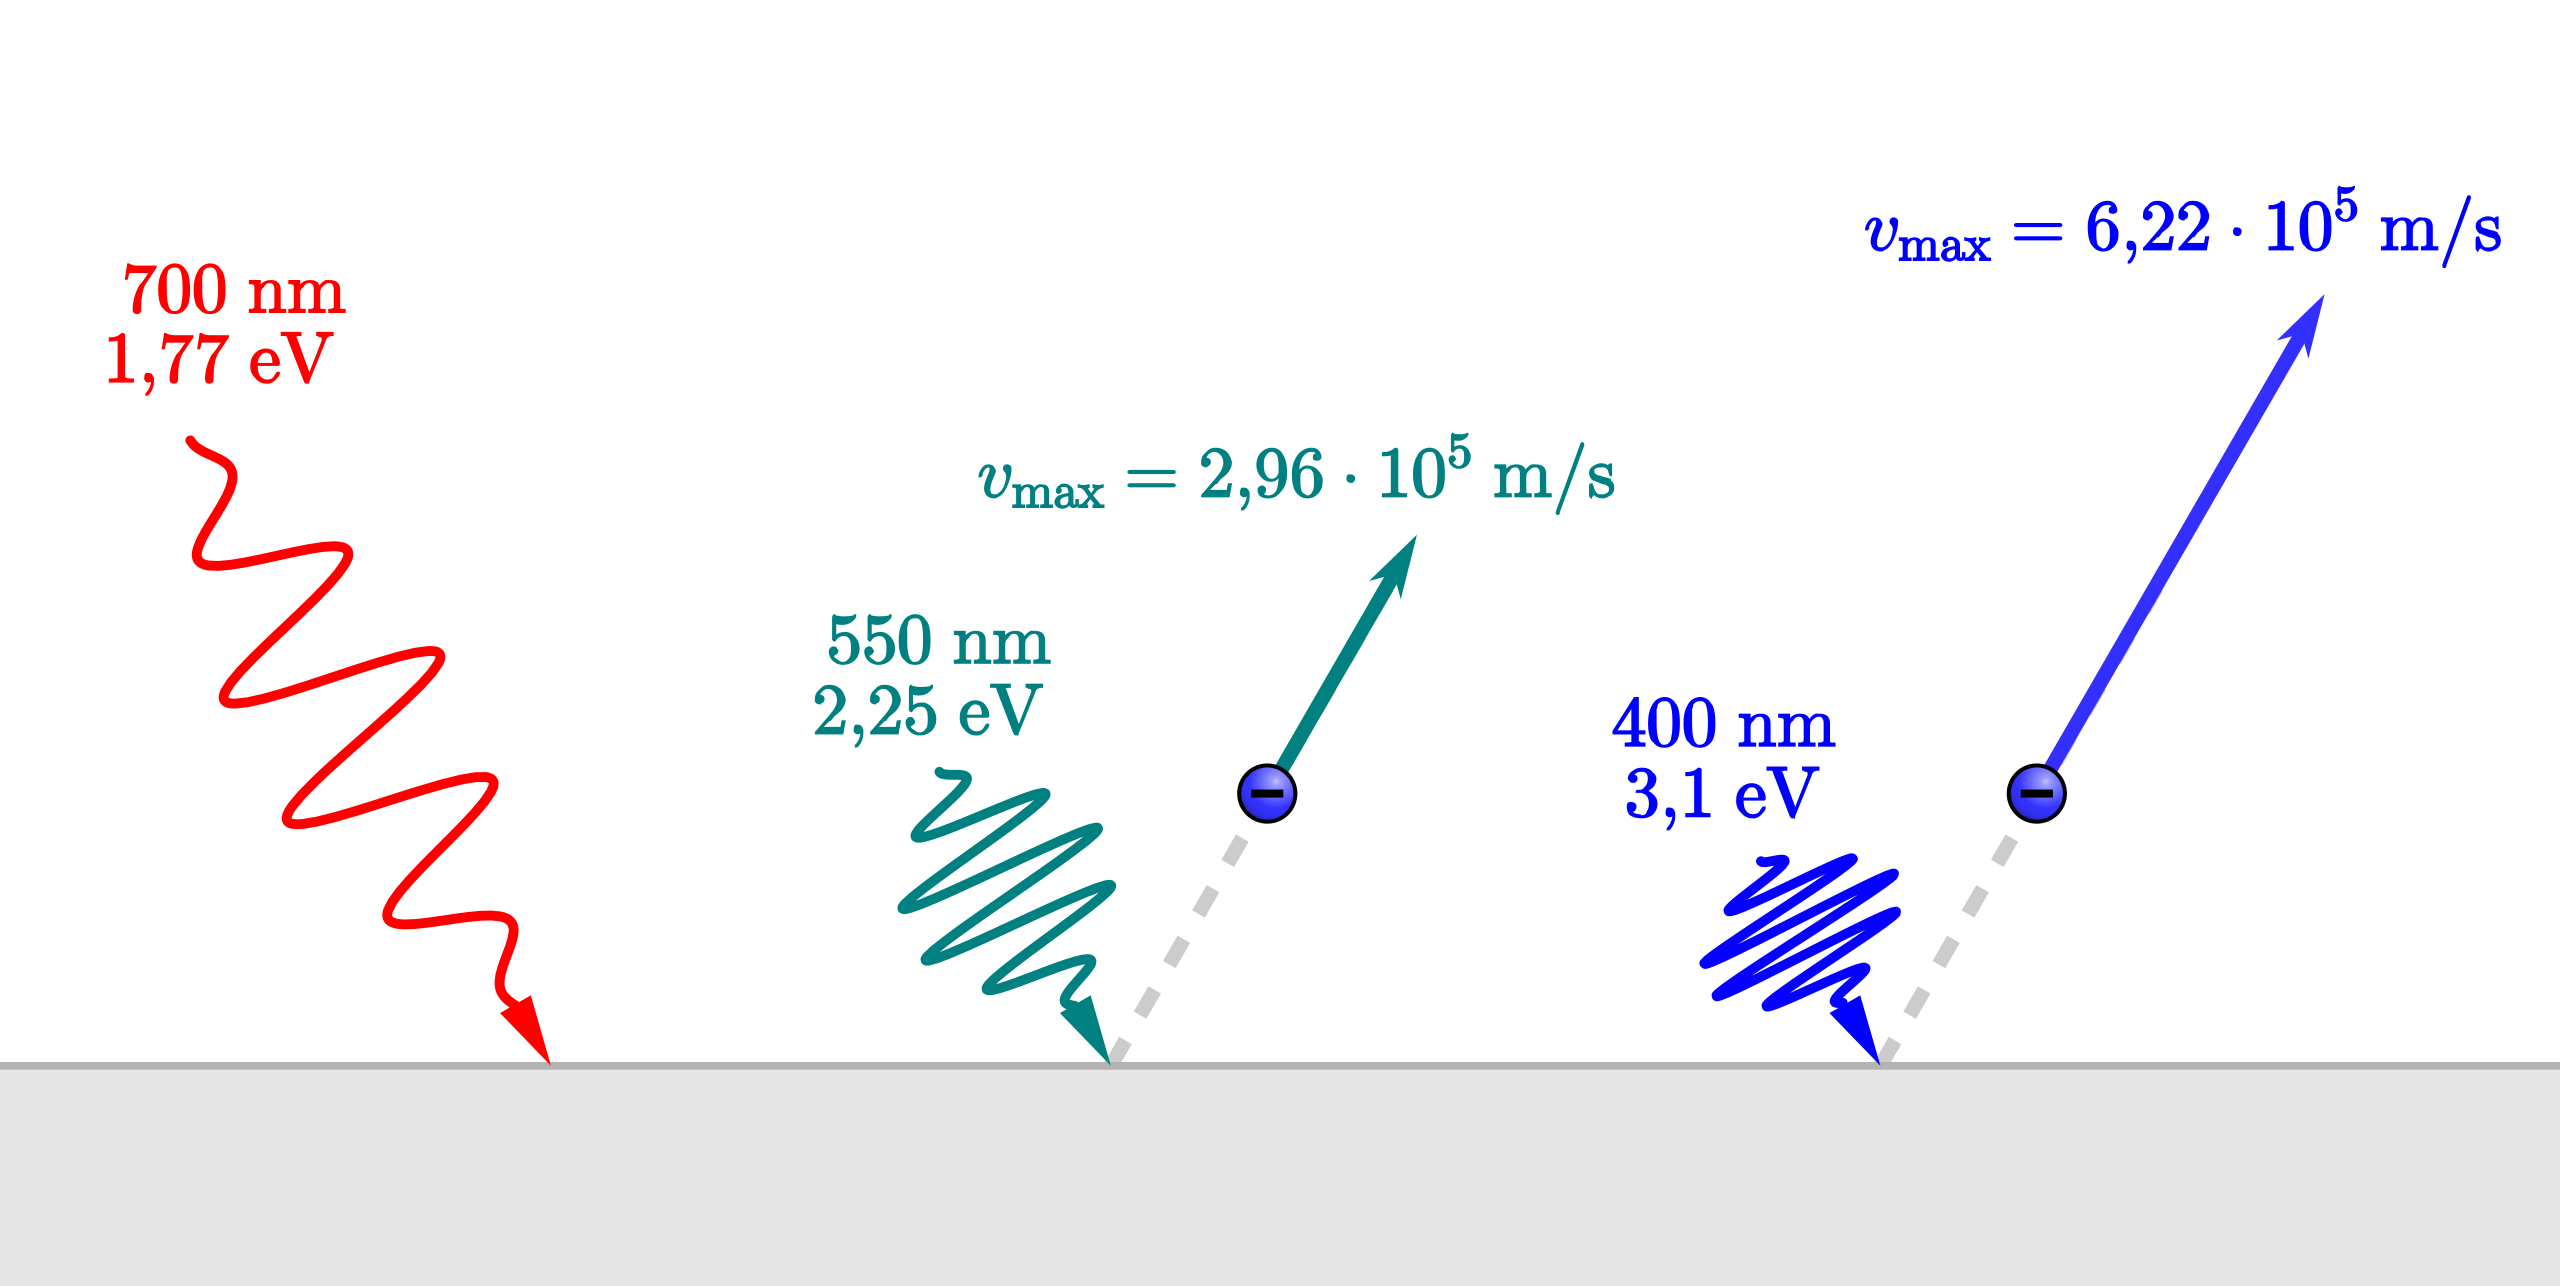
\includegraphics[clip, width=0.6\textwidth]{photoelectric.png}
    \caption{\label{fig:photoelectric} Photoelectric effect. Only certain frequencies allow the ejection of an electron from the metal plate.}
\end{figure}
  \subsection{Conclusions}
  This experiment determined that the energy transfer depends on the frequency $\nu$ of the electromagnetic radiation.
  Moreover, electrons can only acquire certain quanta of energy.
  This led to the introduction of two pivotal concepts of modern physics.

    \subsubsection{Energy quantization}
    The amount of energy transfer to a bound system cannot be arbitrary small.

    \subsubsection{Photons}
    Light is made by the photon particle which carries energy $E = \hbar\nu$, where $\omega = 2\pi\nu$ and $\hbar = \frac{h}{2\pi}$, so:

    $$E = \hbar\omega$$

    Photons, like electrons, share wave-like and particle-like properties.
    Therefore, electrons can be considered as waves of matter and photons as particles of light.

\section{Quantization and atomic spectra}

  \subsection{Experiment}
  A beam of light goes through an atom and a prism.
  The prism splits the frequencies and those frequencies are collected on a screen.
\begin{figure}[h!]
    \centering
    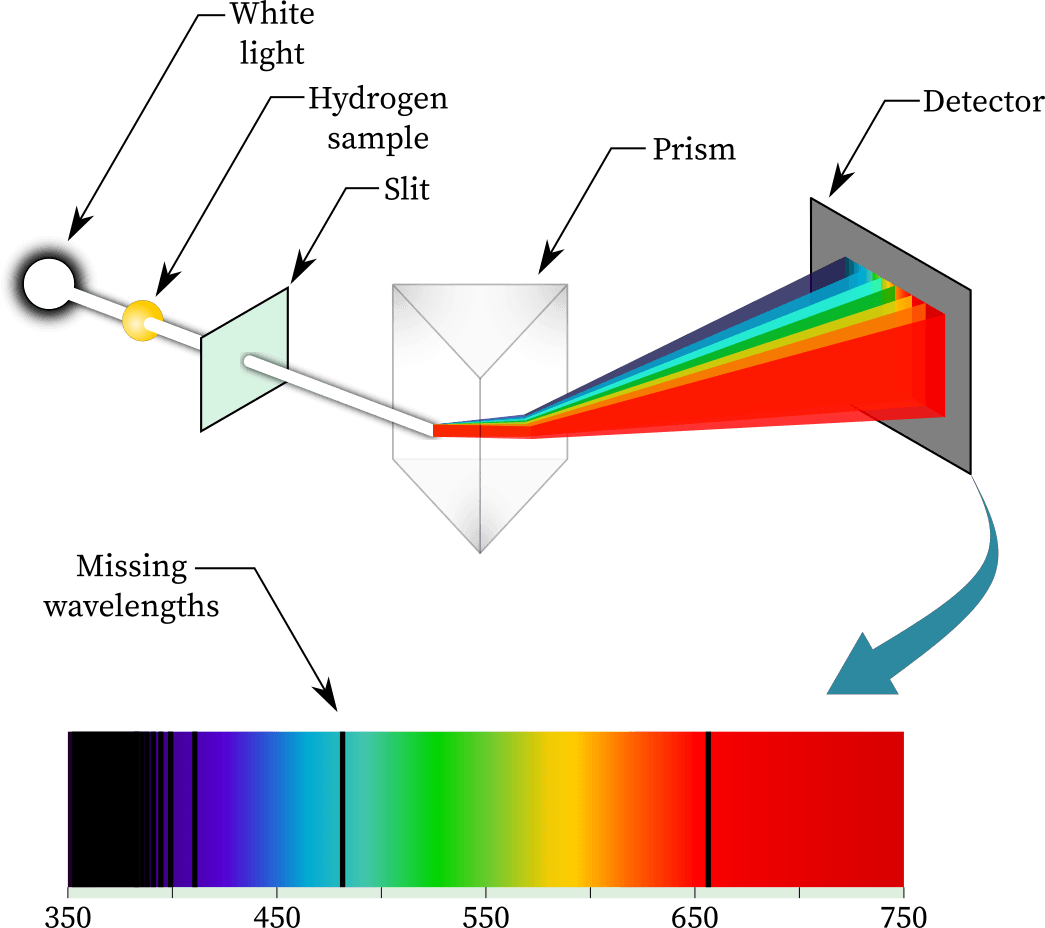
\includegraphics[clip, width=0.6\textwidth]{quantization.png}
    \caption{\label{fig:quantization} Hydrogen emission spectrum: the bright lines in the spectrum are the wavelengths emitted by the excited sample of hydrogen.}
\end{figure}
  \subsection{Finding}
  By performing this experiment, it has been found that only certain frequencies can be absorbed by atoms.

  \subsection{Conclusion}
  Only certain excitation energies are permitted and those form a characteristic signature of atoms:

  $$\hbar\omega = E_n-E_m$$

  Where $E_n$ and $E_m$ are two energy level of the electron in the atom.
  Because of this finding, classical mechanics can be seen as a non-fundamental theory: it perfectly describes observations in some limited range of length, mass, temperature.
  Any more fundamental theory must contain classical mechanics as an approximation in the macroscopic regime, according to the correspondence principle.

\section{Stern Gerlach experiment}

  \subsection{Experiment}
  An electron beam shoots electrons with different momenta $\vec{\mu}$ through an inhomogeneous magnetic field $SG$.
  Behind this there is a screen that detects those electron. If we shut off the magnetic field, the electrons will not interact with anything and we will obtain a high peak. When we activate a magnetic field, there will be some electrons with magnetic moment aligned with velocity and basically left unchanged, while others will be deflected either up or down. We expect to see a wider distribution as a result.


  \subsection{Finding}
  Classically, the electrons are expected to be bended by $SG$ more or less depending on the orientation of $\vec{\mu}$, with an expected density shaped like a Gaussian with $\mu$ at the middle.
  Since $\hat{z}$ has been selected by $SG_1$, $SG_3$, it would be expected to find only $\mu_z = + \mu_0$. Instead, the final beam contains $\mu_z =\pm \mu_0$.
  In real experiments what we see are two narrow peaks; the position of the peaks is compatible with a scenario in which all particles are completely aligned or completely unti-alinged with the z-axis.
  Somehow, the $z$ component of the magnetic moment is QUANTIZED.
  It can only take maximum or negative maximum values.
  Other atoms provide different shapes e.g. up, down, zero.
  But let’s stick to the case in which we observe two peaks.
  Suppose that now we insert a second device aligned to the x-axis.
  This time we are measuring the x-component of the magnetic field.
  Not only the $z$ component is quantised, but also the $x$ and $y$ components.

  \begin{multicols}{2}
    \begin{enumerate}
      \item Select $z$ component.
      \item Filter positive $z$ component.
      \item Select $x$ component.
      \item Filter positive $x$ component.
      \item Measure $z$ component.
    \end{enumerate}
  \end{multicols}

  We already measured the $z$ component, so we expect $x$ to be deflected in a single direction. Surprisingly, $x$ will deflect to both positive and negative with equal probability.

\begin{figure}[h!]
    \centering
    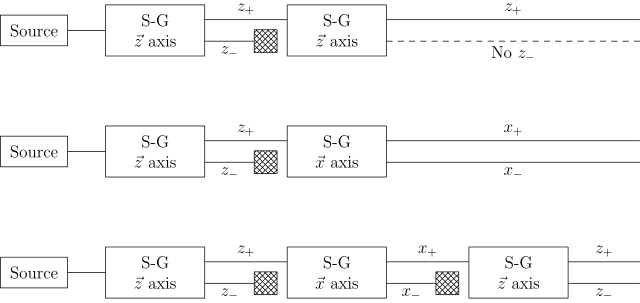
\includegraphics[clip, width=0.6\textwidth]{stern_ger.png}
    \caption{\label{fig:stern_ger} Stern-Gerlach experiment summary}
\end{figure}
  \subsection{Conclusion}
  \underline{The act of measuring $\mu_x$ completely destroys the information about the state of $\mu_z$}.
  According to the uncertainty principle, $\mu_x$ and $\mu_z$ cannot be simultaneously determined.
  Instead, we only find two possible orientations of the magnetic moment, that is in fact quantizied.
  Considering three $SGs$ in series with different orientations: $\hat{z}\rightarrow\hat{x}\rightarrow\hat{z}$:
  The first selects $\hat{\mu}_z = +\mu_0$ and the second $\hat{\mu}_x = +\mu_0$.
  It can be seen, measuring $\mu_z$ in the last $SG$ how the information selected about $\mu_z$ in the first $SG$ is lost.

\section{Finding the Schr\"odinger equation}
Particle propagation is not ballistic:

$$P_{12} \neq P_1 + P_2$$

Probability $P_2$ displayed interference pattern.
Interference pattern naturally arises when taking squared modules of complex amplitudes:

\begin{align*}
  I_{12} &= |A_1 + A_2|^2=\\
         &=(A_1 + A_2)(A_1^*+A_2^*)^*=\\
         &=(A_1A_1^*+\underbrace{A_1A_2^*+A_2A_1^*}_{\text{interference pattern}}A_2A_2^*)
\end{align*}

Considering $E=n\nu$ a wave function for the electron, a propagating wave can be written as:

$$f(x,t) = f_>(x-vt)+f_<(x+vt)$$

And:

\begin{align*}
  \biggl(\frac{1}{v^2}\frac{\partial {^2}}{\partial {t^2}}-\frac{\partial {^2}}{\partial {x^2}}\biggr)\begin{cases}f_>(x+vt)\\f_<(x-vt)\end{cases} &= 0\\
  \frac{1}{v^2}\frac{\partial {}}{\partial {t}}\biggl(\frac{\partial {}}{\partial {t}}f_>(x-vt)\biggr)&-\frac{\partial {}}{\partial {x}}\biggl(\frac{\partial {}}{\partial {x}}f_>(x+vt)\biggr)=\\
  -\frac{1}{v}\frac{\partial {}}{\partial {t}}[f_>'(x-vt)]&=f''_>(x-vt)\\
  f_>''(x-vt) &=f''_>(x-vt)
\end{align*}

Now an electron is assumed to propagate as a wave $\psi(x.t)$ for which: $|\psi(x,t)|^2 = P(x,t)$.
Trying to apply a photon wave to the electron:

$$\psi(x,t) = A_oe^{i(vt-kx)} = \cos(vt-kx) + i\sin(vt - kx)$$

Considering that both the real and imaginary part oscillate:

\begin{align*}
  \begin{cases}\frac{\partial {^2}}{\partial {t^2}}A_0e^{i(vt-kx)} = A_0(-v^2e^{i(vt-kx)})\\\frac{\partial {^2}}{\partial {x^2}}A_0e^{i(vt-kx)} = A_0(-k^2e^{i(vt-kx)})\end{cases}&\rightarrow \frac{1}{\nu^2}\biggl[-A_0v^2e^{i(vt-kx)}+A_0k^2e^{i(vt-kx)}\biggr] = 0\\
                                                                                                                                                                                  &\Rightarrow \nu = v^2k^2\text{ frequency or velocity of propagation}
\end{align*}

From this it can be seen that $E=\nu h\propto v$, but because of the mass of the electron it should be that $E\propto v^2$.
So the Schr\"odinger equation is a modified wave equation to accomodate this:

$$ia \frac{\partial {}}{\partial {t}}\psi=-b \frac{\partial {^2}}{\partial {x^2}}\psi(x,t)$$

  \subsection{Free particle Schr\"odinger equation}
  In this equation, particle interactions and potential energy are not considered:

  $$i\hbar \frac{\partial {}}{\partial {t}}\psi(x,t) = \frac{\hbar^2}{2m}\frac{\partial {^2}}{\partial {x^2}}\psi(x,t)$$

  \subsection{Complete Schr\"odinger equation}
  By allowing the electron to react, we can introduce the operator $H$ - which is composed by kinetic energy and potential energy component (as the classical Hamiltonian).
  Based on this, we can refer to the operator as Quantum Hamiltonian.
  It can be seen how the potential energy is more important than the force:

  $$i\hbar \frac{\partial {}}{\partial {t}}\psi(x,t) = \overbrace{\biggl[-\underbrace{\frac{\hbar^2}{2m}\frac{\partial {^2}}{\partial {x^2}}}_{\text{kinetic energy operator}}+\underbrace{\hat{U}(x)}_{\text{quantum energy operator}}\biggr]}^{\text{Quantum Hamiltonian}}\psi(x,t) = \hat{H}\psi(x,t)$$

  This is a partial differential equation describing the evolution over time of the wave function.
  Uncertainty is reflected by the fact that we do not talk about a space trajectory.
  The interpretation is stochastic ,as the wave function is a probability.
  Therefore, quantum mechanics is not about the nature itself, but rather about predicting the outcomes of experiments on nature.
  The entire foundation of quantum mechanics is computing the probability for an outcome of an experiment.
